\documentclass{beamer}

\usepackage[utf8]{inputenc}
\usecolortheme{beaver}
\usepackage{caption}
\usepackage{subcaption}
\usepackage{mathtools}
\usepackage{todonotes}
\usepackage{amsmath}
\usepackage{bm}
\usepackage{listings}
\usepackage{ragged2e}
\usepackage{titlecaps}
\usepackage{fancyvrb}

\def\ci{\perp\!\!\!\!\!\perp}

\newtheorem{proposition}{Proposition}
\Addlcwords{for a is but and with of in as the etc on to if}

\setbeamertemplate{section in toc}{\inserttocsectionnumber.~\inserttocsection}
\usetheme{Boadilla}
\makeatletter
\setbeamertemplate{footline}{%
    \leavevmode%
    \hbox{%
        \begin{beamercolorbox}[wd=.3\paperwidth,ht=2.25ex,dp=1ex,center]{author in head/foot}%
            \usebeamerfont{author in head/foot}\insertshortauthor\expandafter\beamer@ifempty\expandafter{\beamer@shortinstitute}{}{~~(\insertshortinstitute)}
        \end{beamercolorbox}%
        \begin{beamercolorbox}[wd=.55\paperwidth,ht=2.25ex,dp=1ex,center]{title in head/foot}%
            \usebeamerfont{title in head/foot}\insertshorttitle
        \end{beamercolorbox}%
        \begin{beamercolorbox}[wd=.15\paperwidth,ht=2.25ex,dp=1ex,right]{date in head/foot}%
            \usebeamerfont{date in head/foot}\insertshortdate{}\hspace*{2em}
            \insertframenumber{} / \inserttotalframenumber\hspace*{2ex} 
        \end{beamercolorbox}}%
        \vskip0pt%
    }
\makeatother


\begin{document}

\title[]{Causal Reasoning and Large Language Models: Opening a New Frontier for Causality}
\author {}
\date{}

\begin{frame}
	\begin{figure}
		\centering
		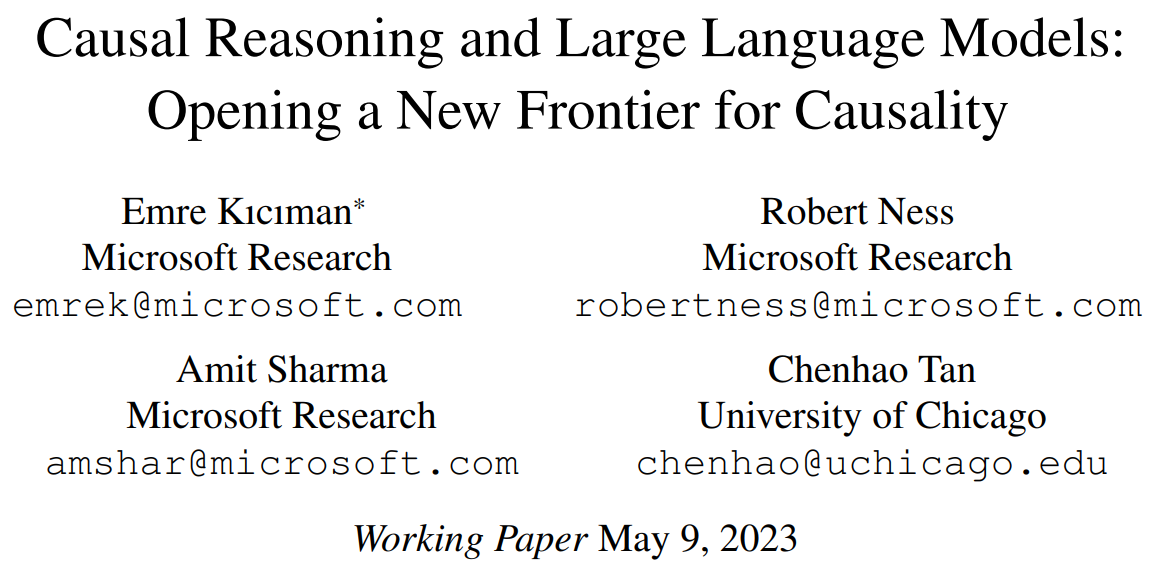
\includegraphics[scale=0.7]{imgs/title.png}
	\end{figure}
\end{frame}

% \begin{frame}
% 	\frametitle{Abstract}
% 	\begin{enumerate}
% 		\item LLM-Based methods establish new state-of-the-art accuracy on multiple causal benchmarks.
% 		\item Outperforms existing algorithms on: 1) Pairwise causal discovery, 2) Counterfactual Reasoning, 3) Actual causality
% 		\item But exhibits unpredictable failure modes.
% 		\item Envisons LLMs to be used alongside existing causal
% 			methods, as a proxy for human domain knowledge.
% 		\item Also see existing causal methods as promising tools for LLMs to
% 			formalize, validate, and communicate their reasoning.
% 		\item Paper doesn't imply that complex causal reasoning has
% 			emerged in LLMs. But it has captured common sense and
% 			domain knowledge from natural language.
% 	\end{enumerate}
% \end{frame}

% \begin{frame}
% 	\frametitle{Introduction}
% 	\begin{enumerate}
% 		\item Paper explores what kind of causal reasoning might LLMs
% 			be performing, if they are, what are the purposes for
% 			which they might be employed, if they can be?
% 		\item Proposes a framework for future research at the intersection of
% 			LLMs and causality.
% 		\item Begins with a recognition of different kinds of causal knowledge 
% 			and reasoning implicated in this debate, including prior knowledge
% 			of general and domain-specific knowledge.
% 		\item Claims that LLMs bring significant new capabilities which
% 			are complementary to existing causal methods.
% 	\end{enumerate}
% \end{frame}

\begin{frame}
	\frametitle{Summary}
	\begin{itemize}
		\item Applying LLMs to causality tasks.
		\begin{enumerate}
			\item Causal Discovery
				\begin{itemize}
					\item Pairwise causal discovery
					\item Full graph discovery
				\end{itemize}
			\item Actual Causality
				\begin{itemize}
					\item Counterfactual reasoning
					\item Necessary and sufficient causes.
					\item Infering normality.
				\end{itemize}
		\end{enumerate}
		\item LLMs perform better or comparable on all these tasks but also make simple, unpredictable mistakes.
		\item Implications and possible future research directions.
	\end{itemize}
\end{frame}


% \begin{frame}
% 	\frametitle{Background: Types of Causality}
% 	\begin{enumerate}
% 		\item Covariance-based Causality: Uses statistical
% 			approaches to discover and estimate the strengths of
% 			causal relationships from data. E.g. Drug efficacy, effects 
% 			of novel economic policies
% 		\item Logic-Based Causality: Fields like law, forensics, fault diagnosis
% 			often emphasize logic-based causality, which uses logical
% 			reasoning and domain knowledge to reason about the causal 
% 			relationships in systems.
% 		\item Type and Actual Causality: Type causality encompasses inference
% 			on causal relationships between variables, such as in causal 
% 			discovery and causal effect estimatio. In contrast, actual 
% 			causality refers to inference of the degreee to which specific
% 			events cause other events. Questions like "Was Fred's smoking 
% 			habit responisble for his lung cancer?"
% 	\end{enumerate}
% \end{frame}
% 
% \begin{frame}
% 	\frametitle{Background: Different Causal Tasks and their connections to kinds of causality}
% 	Some of the causal inference tasks.
% 	\begin{enumerate}
% 		\item Causal Discovery: The task of recovering the underlying causal
% 			mechanism that govern a system. Primarly covariance-based in the
% 			context of type causality.
% 		\item Effect Inference: Task of characterizing the strength and shape of 
% 			a known or hypothesized causal relationship. \todo[inline]{Maybe add more to this}
% 		\item Attribution: Task of determining the cause of a change. Depending on the applicatio domain, usually involves both covariance based and logic based approaches.
% 		\item Judgement tasks: Extend attribution tasks to question of reward or
% 			blame assignment for outcomes.
% 	\end{enumerate}
% \end{frame}
% 
% \begin{frame}
% 	\frametitle{LLMs and Causality}
% 	\begin{enumerate}
% 		\item First, the paper investigates the graph discovery capabilities of
% 			LLMs over a broad set of complex real-world tasks.
% 		\item Second, the paper probes the ability of LLMs to do counterfactual
% 			reasoning and infer necessary or sufficient cause based on
% 			natural language description of the world.
% 	\end{enumerate}
% \end{frame}
% 
% \begin{frame}
% 	\frametitle{Probing LLM behaviors}
% 	\begin{enumerate}
% 		\item Since LLMs are text based, the main way to understand its causal
% 			capibiilities is to probe it with different inputs and observe
% 			how the output changes.
% 		\item This paradigm has the classic limitation of construct
% 			validity for the measurements. That is we may be
% 			tempted to ascribe a particular causal capability to an
% 			LLM if it answers well on a set of questions related to
% 			the capability.
% 		\item Tests the capabiility on standard benchmark datasets and also
% 			does memoization tests on the LLM to test the extent to which
% 			the LLM has memoized the benchmark. Construct novel datasets, and
% 			do perturbations to test whether the LLM is memoizing.
% 	\end{enumerate}
% \end{frame}
% 
% \begin{frame}
% 	\frametitle{Benchmark Tests and Question-Answer Evaluation}
% 	\begin{enumerate}
% 		\item Give a prompt to the LLM and the completion of the prompt is 
% 			the answer.
% 		\item For each evaluation, we ask a series of questions or causal 
% 			challenges and score the correctness of the resulting answer.
% 	\end{enumerate}
% \end{frame}
% 
% \begin{frame}
% 	\frametitle{Memorization Test}
% 	\begin{enumerate}
% 		\item The primary treat to the validity of benchmark or question-answer
% 			style assessments is that the LLM may have directly 
% 			memorized the benchmark answers.
% 		\item To test whether the LLM has memorized a particular dataset
% 			or benchmark, we give the LLM a partial row of data from
% 			the dataset and ask it to complete the remaining.
% 		\item For question-answer taks half of the question and ask it to 
% 			complete the rest.
% 		\item To encourage the LLM to succeed, we prepend details about the
% 			dataset, such as its name, URL, and description, and also
% 			provide few-shot examples.
% 	\end{enumerate}
% \end{frame}
% 
% \begin{frame}
% 	\frametitle{Redaction Test}
% 	\begin{enumerate}
% 		\item To better understand what aspets of the prompt or
% 			question an LLM is attending to, we use redaction and
% 			perturbation tests.
% 		\item First, we redact words in the prompt, one by one, and see how 
% 			the answers change each time. Changes in the answer indicate
% 			the LLM is attending to the redacted word.
% 	\end{enumerate}
% \end{frame}
% 
% \begin{frame}
% 	\frametitle{LLMs and Causal Discovery}
% 	\begin{enumerate}
% 		\item Having the correct causal graph that encodes causal assumptions
% 			is critical for ensuring the correctness of any downstream
% 			analysis.
% 		\item Generally it is not possible to learn the correct graph for
% 			a given dataset, given only observational dataset.
% 		\item A set of graph structures known as Markov Equivalence
% 			class are equally likely given the same observational
% 			data distribution.
% 		\item Two main approaches to overcome this issue:
% 			\begin{itemize}
% 				\item Restrict data-generating process to a specific
% 					functional form under which identification
% 					of a single graph is possible.
% 				\item Use deep learning to model the covariances of
% 					all variables jointly and hope that it improves
% 					the quality of learned graphs.
% 			\end{itemize}
% 		\item LLMs offer a fresh perspective on the causal discovery problem
% 			by focusing on the metadata associated with variables in a 
% 			dataset, rather than their data values.
% 		\item Usually domain experts can use such meta data along with the 
% 			context to construct causal structures. LLM does the same 
% 			thing.
% 	\end{enumerate}
% \end{frame}

\begin{frame}
	\frametitle{Pairwise Causal Discovery: T\"{u}bingen Cause-effect Pairs Dataset}
	\begin{itemize}
		\item Given a dataset on $ 2 $ variables, determine the direction of causality.
			$$ (X, Y) \implies X \rightarrow Y \;\; \textit{or} \; \; X \leftarrow Y $$
		\item 108 cause-effect pairs selected from 37 datasets from
			various domains.
	\end{itemize}
	\begin{figure}
		\centering
		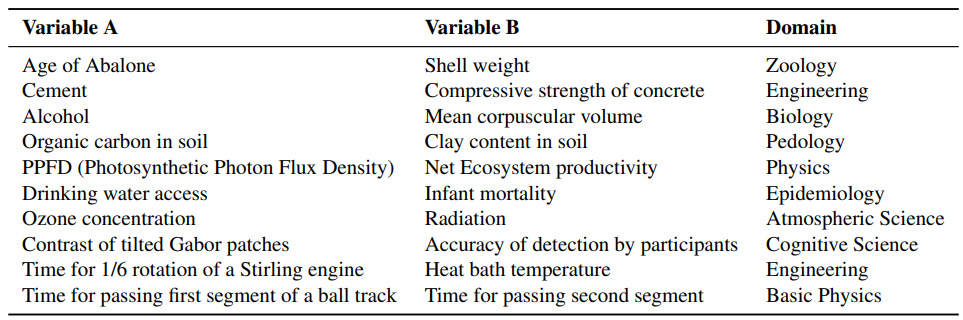
\includegraphics[scale=0.45]{imgs/table1.png}
	\end{figure}
\end{frame}

\begin{frame}
	\frametitle{Pairwise Causal Discovery: T\"{u}bingen Cause-effect Pairs Dataset}
	\begin{enumerate}
		\item \textbf{Two prompts: } Query in both directions: Does changing A cause a change in B? Does chaning B cause a change in A?
		\item \textbf{Causal agent: } Prepend the prompt with "You are a helpful assistant for causal reasoning"
		\item \textbf{Single Prompt: } Ask to output the more likely causal direction while explaining the reasoning.
	\end{enumerate}
	\begin{figure}
		\centering
		\begin{subfigure}{0.5 \textwidth}
			\centering
			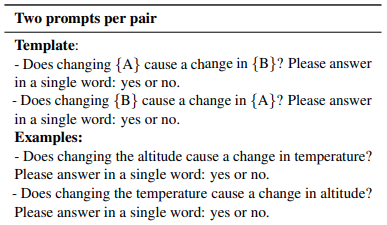
\includegraphics[scale=0.4]{imgs/example1.png}
		\end{subfigure}%
		\begin{subfigure}{0.5 \textwidth}
			\centering
			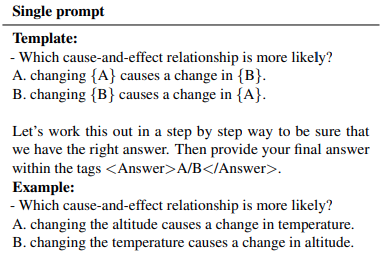
\includegraphics[scale=0.4]{imgs/example2.png}
		\end{subfigure}
	\end{figure}
\end{frame}

\begin{frame}
	\frametitle{Pairwise Causal Discovery: T\"{u}bingen Cause-effect Pairs Dataset}
	\begin{columns}
		\begin{column}{0.5 \textwidth}
			\begin{itemize}
				\item Results are dependent on the prompt used.
				\item LLMs can give wrong results because of ambiguity in the variable names. E.g., (Ozone concentration, radiation).
				\item Providing context can result in getting the correct answer.
			\end{itemize}
		\end{column}
		\begin{column}{0.5 \textwidth}
			\begin{figure}
				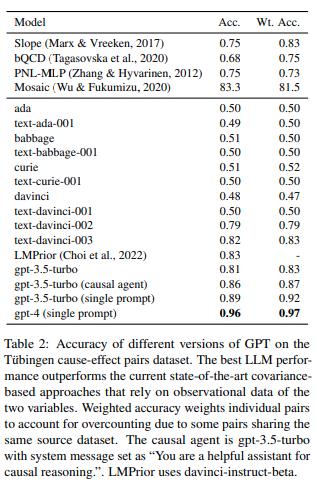
\includegraphics[scale=0.2]{imgs/table2.png}
			\end{figure}
		\end{column}
	\end{columns}
\end{frame}

\begin{frame}
	\frametitle{Pairwise Causal Discovery: Neuropathic Pain Dataset}
	\begin{itemize}
		\item The variable names are more domain specific.
		\item Dataset contains relationship between different nerves and the associated symptoms that patients express.
	\end{itemize}
	\begin{figure}
		\centering
		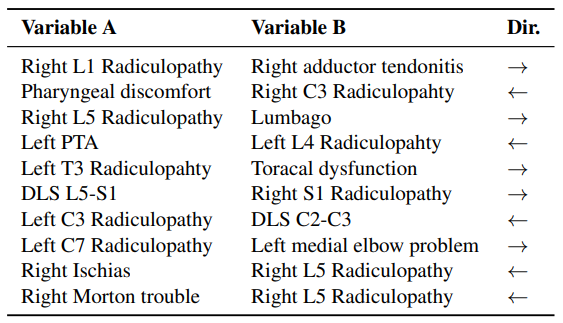
\includegraphics[scale=0.6]{imgs/table3.png}
	\end{figure}
\end{frame}

\begin{frame}
	\frametitle{Pairwise Causal Discovery: Neuropathic Pain Dataset}
	\begin{columns}
		\begin{column}{0.5 \textwidth}
			\begin{itemize}
				\item Performance of text generation engines degrade but chat-based models perform well.
			\end{itemize}
		\end{column}
		\begin{column}{0.5 \textwidth}
			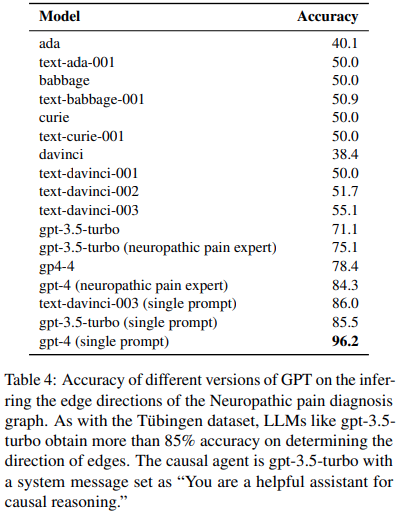
\includegraphics[scale=0.25]{imgs/table4.png}
		\end{column}
	\end{columns}
\end{frame}

\begin{frame}
	\frametitle{Full Graph Discovery}
	\begin{itemize}
		\item Given a dataset, find a DAG representing the causal relationships between the variables.
		\item Three possible scenario between any two variables: $ X \rightarrow Y $, $ X \leftarrow Y $, or no edge.
		\item Need to also distinguish between direct and indirect effects.
		\item If true relationship is $ A \rightarrow B \rightarrow C $, for pairwise task correct to output $ A \rightarrow B $
			and $ A \rightarrow C $, but not for full graph discovery.
		\item Unclear how to extend pairwise task to a full graph case.
		\item For smaller graphs with 3-4 variables, can iterate over all possible pairs of variables.
	\end{itemize}
\end{frame}

\begin{frame}
	\frametitle{Full Graph: Neuropathic Pain Dataset}
	\begin{itemize}
		\item The dataset has 221 variables; not possible to do a full graph discovery.
		\item Utilize a smaller 100 pair dataset. 50 pairs form edges in the graph and 50 pairs do not form an edge.
		\item In the single prompt an additional option is added as: ``C: No causal relationship exists''.
	\end{itemize}
	\begin{figure}
		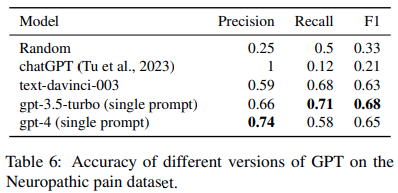
\includegraphics[scale=0.4]{imgs/table6.png}
	\end{figure}
\end{frame}

\begin{frame}
	\frametitle{Full Graph: Arctic Sea Ice Dataset}
	\begin{itemize}
		\item Dataset on driver of arctic sea ice thickness/coverage.
		\item Total of 12 variables and 48 edges with some double-sided edges.
		\item Only ``single prompt'' used for LLMs.
	\end{itemize}
	\begin{figure}
		\centering
		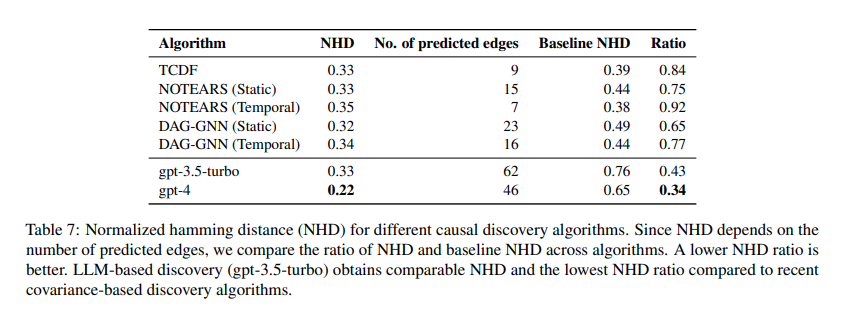
\includegraphics[scale=0.42]{imgs/table7.png}
	\end{figure}
\end{frame}

\begin{frame}
	\frametitle{Probing LLM Behavior: Memorization Test}
	\begin{itemize}
		\item Test whether the LLMs have memorized the benchmark datasets.
		\item Provide LLM with the first 3 columns of the dataset
			(row ID and two variables) and ask it to complete the
			remaining columns.
		\item GPT-3.5 and GPT-4 correctly recall 19\% and
			25\% of the rows. 
		\item Significant gap between percentage memorized and LLM's
			accuracy.
		\item Expect LLMs to be partially dependent on memorization but
			partially able to process and transform seen causal
			relationships in multiple context.
	\end{itemize}
\end{frame}

\begin{frame}
	\frametitle{Probing LLM Behavior: Redaction Test}
	\begin{itemize}
		\item Redact words one-by-one and check how important they are for making the correct decision.
	\end{itemize}
	\begin{figure}
		\centering
		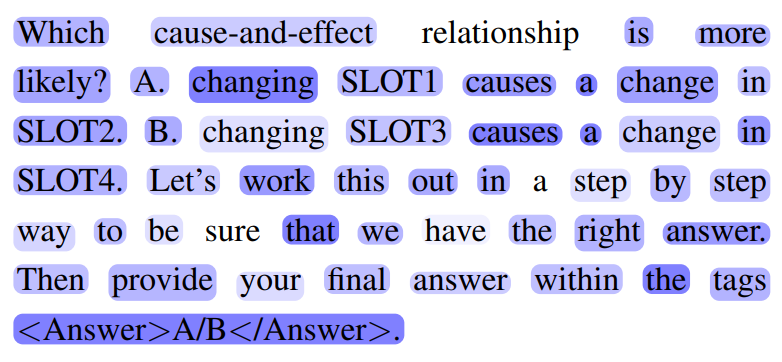
\includegraphics[scale=0.4]{imgs/figure4.png}
	\end{figure}
\end{frame}

% \begin{frame}
% 	\frametitle{LLMs for Actual Causality and Causal Judgments}
% 	\begin{itemize}
% 		\item Actual causality is motivated by problems of attribution and assigning responsibility in real world applications, such as legal reasoning,
% 			machine failure debugging, and root-cause analysis for system regressions.
% 		\item SCMs and other formal causal methods have been used to define actual causality in a way that is consistent with how humans 
% 			naturally attribute cause and related concepts.
% 		\item Things that are difficult to formalize with SCMs.
% 		\begin{enumerate}
% 			\item Causal Frame: The set of candidate causal events that are relevant to a particular outcome event.
% 			\item Necessary Causality: Whether a candidate cause needed to happen for the outcome to occur.
% 			\item Sufficient causality: Whether a candidate cause's occurance would have led to the outcome event if other causal events had 
% 				occured differently.
% 			\item Normality: The degree to which causal events align with statistical norms or prescriptive norms.
% 			\item Other human factors: Other human factors include bias towards action, handling intention and epistemic state, and how
% 				bad outcomes are interpreted.
% 		\end{enumerate}
% 	\end{itemize}
% \end{frame}

\begin{frame}
	\frametitle{Counterfactual Reasoning}
	\begin{itemize}
		\item Considering hypothethical situations or alternate
			realities by altering specific conditions of an actual
			event. What-if questions.
		\item CRASS (Counterfactual Reasoning Assessment) dataset for
			evaluating the ability of LLMs to answer counterfactual
			conditonal questions.
	\end{itemize}
	\begin{figure}
		\centering
		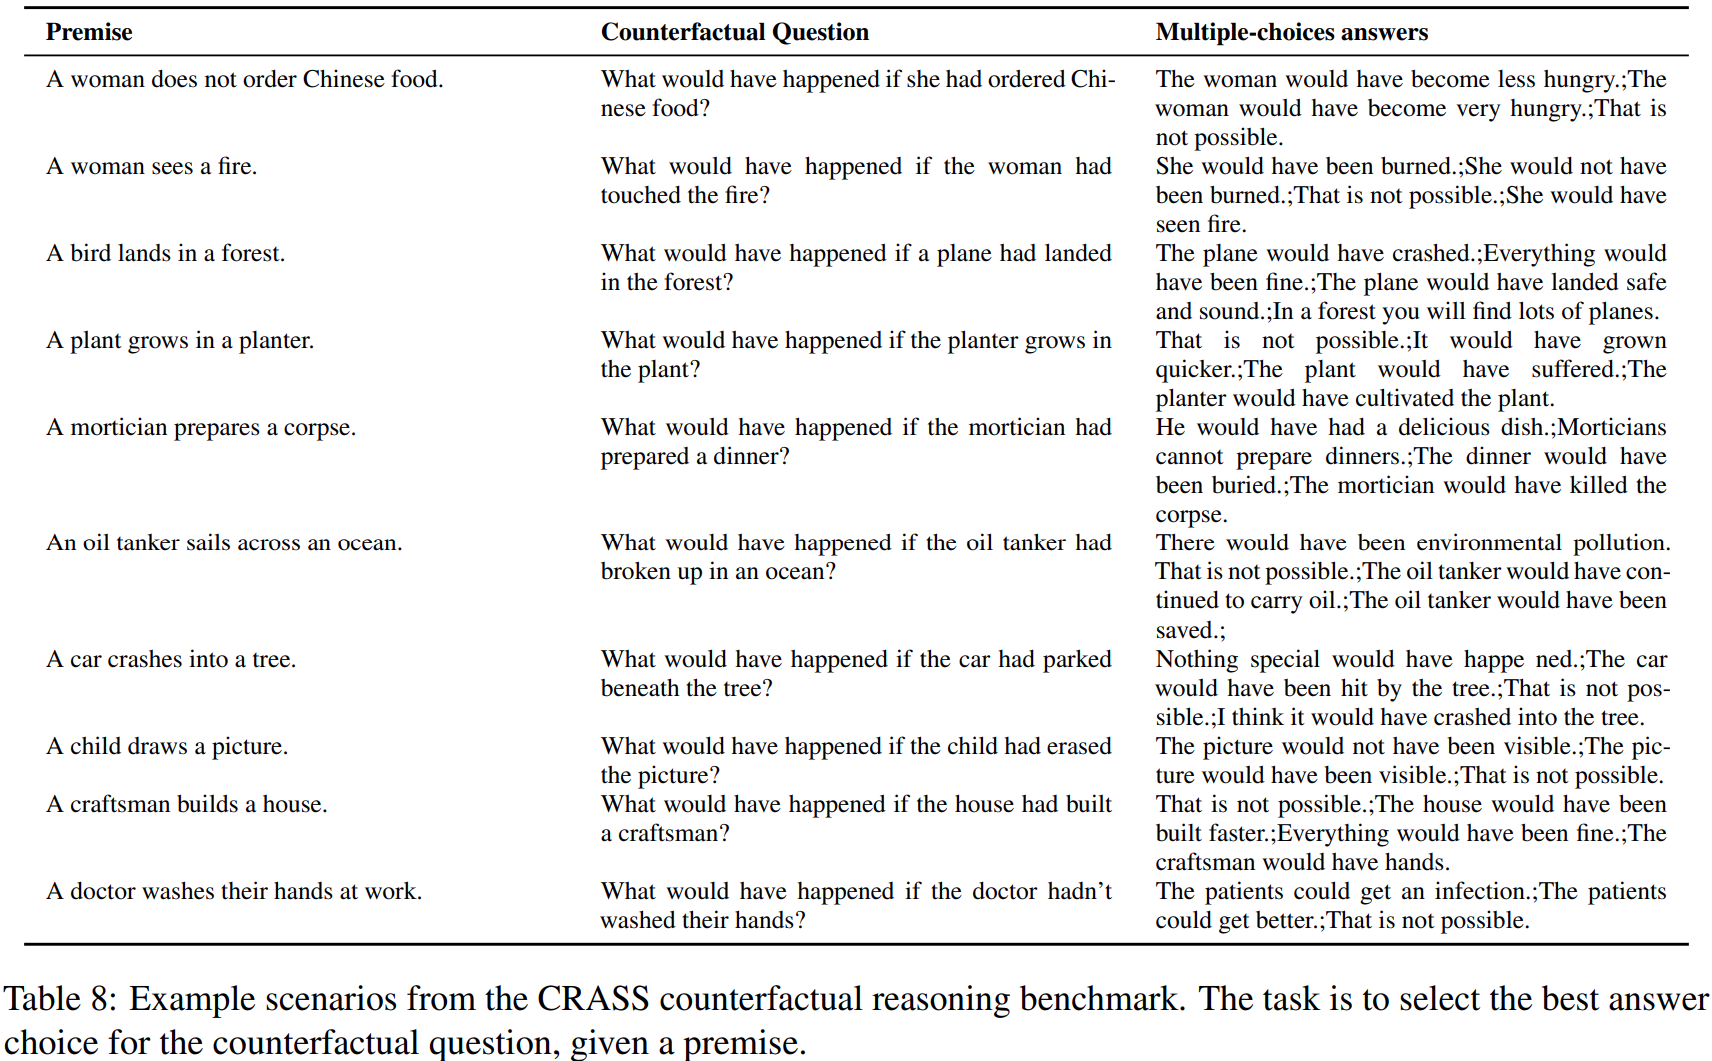
\includegraphics[scale=0.22]{imgs/table8.png}
	\end{figure}
\end{frame}

\begin{frame}
	\frametitle{Counterfactual Reasoning}
		\begin{figure}
			\centering
			\begin{subfigure}{\textwidth}
				\centering
				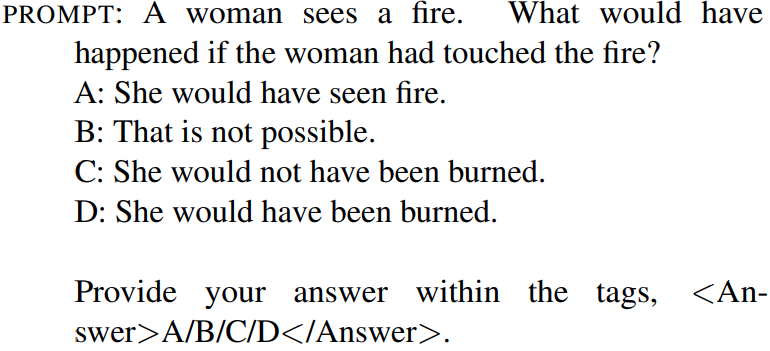
\includegraphics[scale=0.25]{imgs/counter_promp.png}
			\end{subfigure}\vspace{1em}
			\begin{subfigure}{\textwidth}
				\centering
				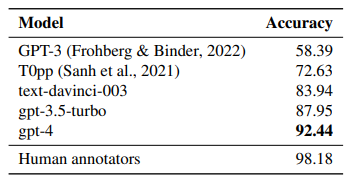
\includegraphics[scale=0.7]{imgs/table9.png}
			\end{subfigure}
		\end{figure}
		\begin{itemize}
			\item Not always sure about the output. Adding context helps.
		\end{itemize}
\end{frame}

\begin{frame}
	\frametitle{Counterfactual Reasoning: Understanding LLM output}
	\begin{columns}
		\begin{column}{0.5\textwidth}
			\begin{figure}
				\begin{subfigure}{\textwidth}
					\centering
					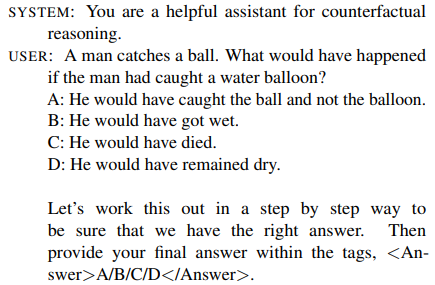
\includegraphics[scale=0.55]{imgs/counterfactual_prompt1.png}
				\end{subfigure}
				\begin{subfigure}{\textwidth}
					\centering
					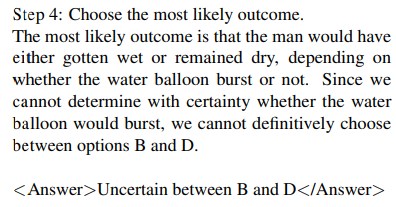
\includegraphics[scale=0.55]{imgs/counterfactual_prompt2.png}	
				\end{subfigure}
			\end{figure}
		\end{column}
		\begin{column}{0.5\textwidth}
			\begin{figure}
				\begin{subfigure}{\textwidth}
					\centering
					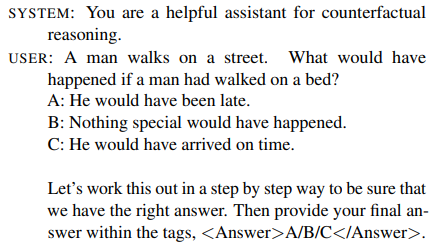
\includegraphics[scale=0.55]{imgs/counterfactual_prompt3.png}
				\end{subfigure}
				\begin{subfigure}{\textwidth}
					\centering
					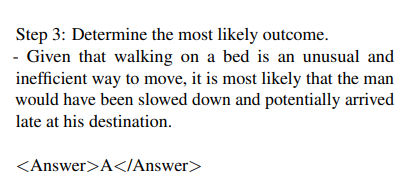
\includegraphics[scale=0.55]{imgs/counterfactual_prompt4.png}	
				\end{subfigure}
			\end{figure}
		\end{column}
	\end{columns}
\end{frame}

\begin{frame}
	\frametitle{Necessary and Sufficient Causes}
		\begin{columns}
			\begin{column}{0.5 \textwidth}
				\begin{figure}
					\centering
					\begin{subfigure}{\textwidth}
						\centering
						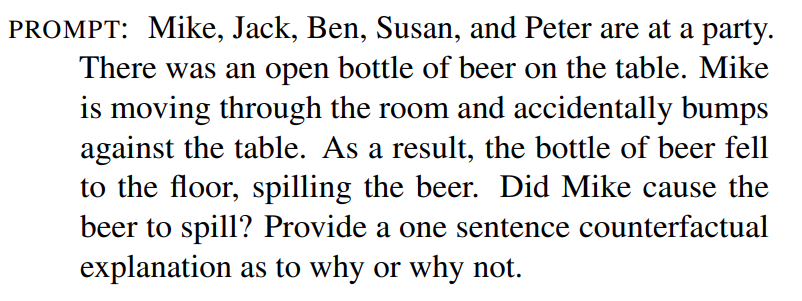
\includegraphics[scale=0.22]{imgs/necessary_prompt_1.png}
					\end{subfigure}
					\begin{subfigure}{\textwidth}
						\centering
						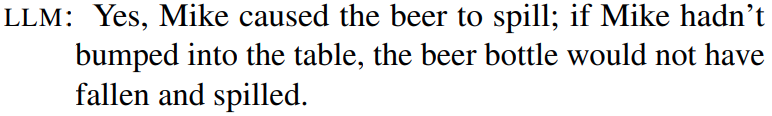
\includegraphics[scale=0.22]{imgs/necessary_prompt_llm.png}
					\end{subfigure}
					\caption*{\footnotesize Necessary Causality}
				\end{figure}
			\end{column}
			\begin{column}{0.5 \textwidth}
				\begin{figure}
					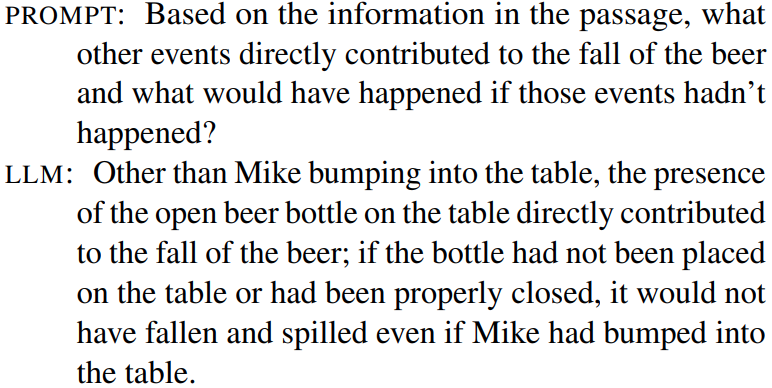
\includegraphics[scale=0.22]{imgs/robust_prompt.png}
					\caption*{\footnotesize Sufficient Causality}
				\end{figure}
			\end{column}
		\end{columns}
		\begin{itemize}
			\item \footnotesize \textbf{Necessary Causality:} The
					property of an event, C, that if it had
					not occurred, then the outcome event,
					E, would not have occurred.
			\item \footnotesize \textbf{Sufficient
					Causality:} Given that causal event C
					occurred, outcome event E would have
					occurred even if other events that
					contributed to E's occurrence had not
					occurred.
		\end{itemize}
\end{frame}

\begin{frame}
	\frametitle{Evaluation Necessary and Sufficient Causes}
	\begin{figure}
		\centering
		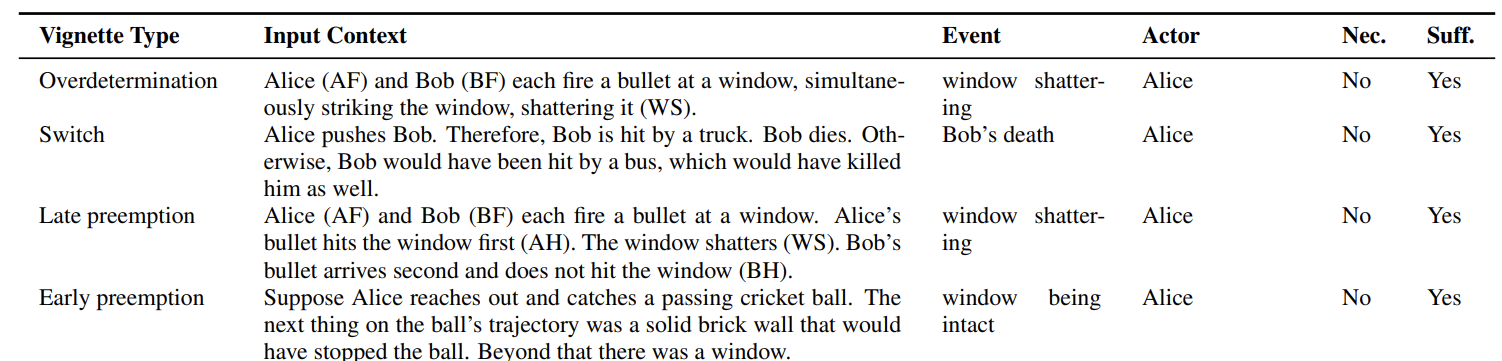
\includegraphics[scale=0.2]{imgs/vignette.png}
	\end{figure}
	\begin{columns}
		\begin{column}{0.5\textwidth}
			\begin{figure}
				\centering
				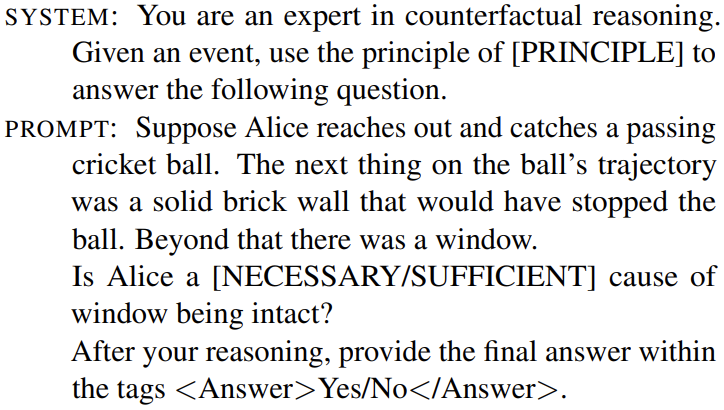
\includegraphics[scale=0.25]{imgs/neccessary_prompt.png}
			\end{figure}
		\end{column}
		\begin{column}{0.5\textwidth}
			\begin{figure}
				\centering
				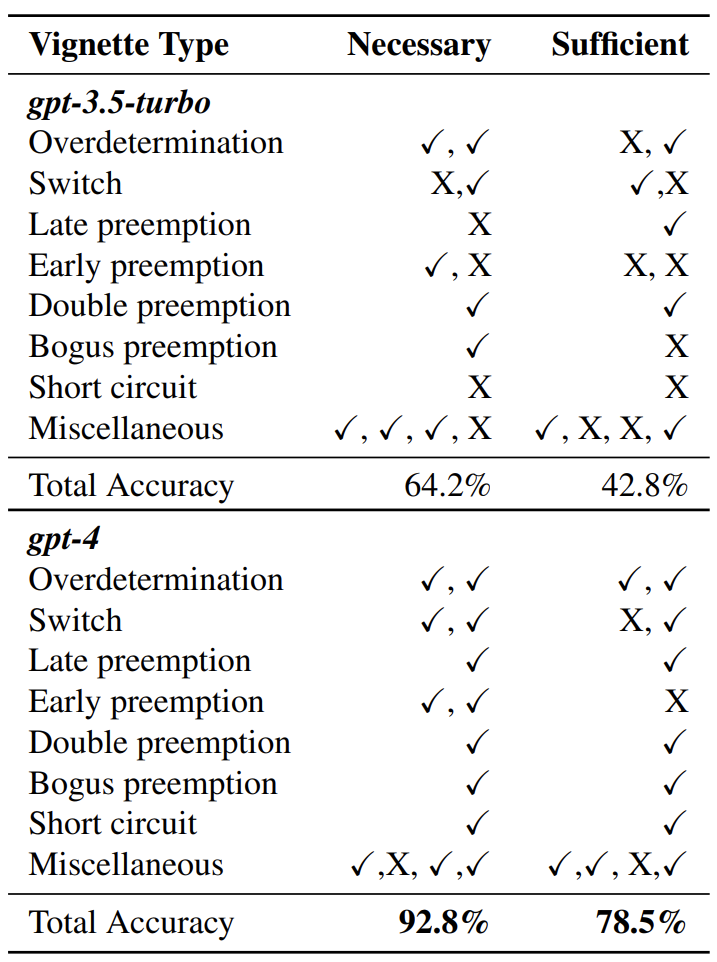
\includegraphics[scale=0.15]{imgs/table_11_12.png}
			\end{figure}
		\end{column}
	\end{columns}
\end{frame}

\begin{frame}
	\frametitle{Inferring Normality}
	\begin{figure}
		\centering
		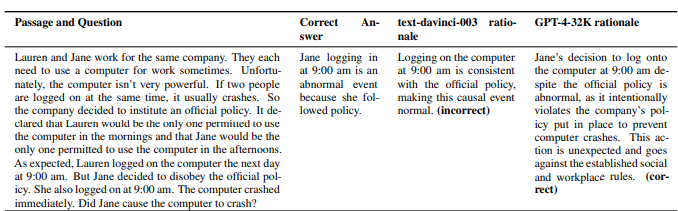
\includegraphics[scale=0.68]{imgs/normality.png}
	\end{figure}
	\begin{itemize}
		\item Event is ``abnormal'' if its occurence was unexpected,
			unlikely, etc. Or event was an agent's action or lack
			of action that knowingly violated social, legal, or
			ethical norms.
		\item First prompt the LLM to extract the causal event in question.
		\item Then ask LLM to evaluate the normality of the causal event in question.
	\end{itemize}
\end{frame}

% \begin{frame}
% 	\frametitle{Implications for causality research}
% 	\begin{enumerate}
% 		\item Conventional causal discovery and effect inference rely strongly on prior domaning knowledge.
% 		\item Current best practice relies on human domain experts to provide this knowledge.
% 		\item Capturing domain knowledge in a formal representation suitable for analysis remains a challenge.
% 		\item LLMs allow access to an array of memorized or inferred causal mechanisms, capturing general and domain-specific knowledge and may augment human experts by aiding in bootstrapping, critiquing, etc.
% 		\item LLMs do have unexpected failure modes. In all the tasks studies, LLMs achive high average accuracies but also make simple, unpredictable mistakes on certain inputs.
% 		\item Accuracy depends on the prompt used.
% 		\item Further research is needed to understand when LLM outputs can be trusted and increase their robustness.
% 	\end{enumerate}
% \end{frame}

\begin{frame}
	\frametitle{Summary}
	\begin{itemize}
		\item LLMs provide access to domain knowledge that was only available
			via human domain experts.
		\item LLMs provide a flexible, natural language-based interaction 
			mechanism for conducting causal analysis that can work
			alongside existing tools.
		\item LLMs offer a new capability to extract the key primitives of
			an actual causality question.
		\item For high-risk and high-value tasks, LLM based approaches would
			need integration with more formal approaches to
			causal reasoning.
	\end{itemize}
\end{frame}

\begin{frame}
	\frametitle{Implications for Causality Practitioners}
	\begin{itemize}
		\item Augmenting human expertise with LLMs
			\begin{itemize}
				\item Can act as assistants for causal discovery and
					doing robustness checks.
				\item Can generate an initial version of
					causal graphs.
			\end{itemize}
		\item LLM + Causal Tools: Pipeline for causal analysis
			\begin{itemize}
				\item LLMs are not capable of replacing tools
					that do statistical analysis for
					estimating causal quantities.
				\item Can construct pipelines where graph creation is
					done by LLMs and final output graph is passed to
					an inference tool.
			\end{itemize}
		\item LLMs as a fluid conversational interface, merging covariance-
			and logic-based reasoning.
	\end{itemize}
\end{frame}

\begin{frame}
	\frametitle{Research Questions: Knowledge-based Causal Discovery}
	\begin{itemize}
		\item Current methods only utilize data but as shown variable
			metadata contains useful information as well.
		\item Developing methods that utilize both.
		\item LLMs can be used as a prior, as a critic during learning, and/or
			as a post-processor.
	\end{itemize}
\end{frame}

\begin{frame}
	\frametitle{Research Questions: LLM-guided Effect Inference}
	\begin{itemize}
		\item Having a correct graphical structure is important for identifying
			correct adjustment set.
		\item Interesting to see if LLMs can be used to suggest
			potential instrumental variables.
		\item Utilizing LLM's domain knowledge to help build robustness
			and validation checks for a given causal analysis.
	\end{itemize}
\end{frame}

\begin{frame}
	\frametitle{Research Questions: Systematizing Actual Causality and Attribution}
	\begin{itemize}
		\item LLMs can be used in such cases for doing root cause analysis and
			credit assignment in domains like law, intelligence analysis, etc.
		\item Hard to formalize common sense background knowledge, LLMs can
			work with these background concepts directly in natural
			language.
	\end{itemize}
\end{frame}

\begin{frame}
	\frametitle{Research Questions: Understanding and Improving Causal Reasoning in LLMs}
	\begin{itemize}
		\item Understanding why LLMs demonstrate such causal capabilities
			as well as the limits of these capabilities. 
		\item According to Pearl's causal hierarchy, LLMs trained on
			observational data should not be able to answer
			interventional or counterfactual queries.
		\item LLMs are potentially learning correlations
			of causal facts from the training data, rather than learning
			to reason causally.
	\end{itemize}
\end{frame}

\end{document}
